
\section{Control}

\subsection{intro}
Today, this kind of operation is done by maneuvring the vehicle to a position where the manipulator is within reach of the hot stab. Once the desired vehicle position is reached, the vehicle is kept stationary by using dynamical positioning, and another operator operates the manipulator arm to do insert the hot stab. The manipulator is normally controlled through a master-slave configuration,\footnote{A master-slave configuration is a control method where an operator moves a replica of the real manipulator. The obtained angles of the replica is then used by the motion control of the manipulator to obtain the same pose as the replica.} 
or through controling the rates of the joints directly. Both these methods suffer from the following drawbacks:

\begin{itemize}
	\item The operator is dependant on high video feedback with very low latency in order to make the correct adjustments of the manipulator.  
	\item Two operators are normally required, one for the vehicle and one for the manipulator arm.
	\item One has to switch between maneuvring the vehicle and the manipulator, even for tasks that are fairly close to eachother, potentially using more energy then required by the task itself. 
	\item Interaction with the environment is difficult due to latency in force feedback from the manipulator, and difficulty in estimating the forces caused by the interaction.
\end{itemize}
One of the objectives of the control strategy is to keep the human operator out of the control loop as much as possible. This makes the system less dependant on high speed telemetry which is important when operating nontethered vehicles, making it possible to control them from a great distance. 
The proposed control structure is based on controlling the motion of the end effector seen from the end effector frame \frame{ee}. Kinematically this will be done by an inverse kinematic strategy mapping the end effector velocities 
to joint, and vehicle velocities, which will be discussed later. This gives the operator the opportunity to ``fly'' the end effector, without dealing with the rest of the manipulator or the vehicle, as this is being managed locally by the control system. 
Lets now identify the main states of operation of the UVMS, which is useful when designing the control system. 

\begin{itemize}
	\item Transport. This state represent the relatively long distance transport of the UVMS to and from a location where it operates, or when doing inspections of e.g. pipelines. This state requires relatively low accuracy in guidance and is typically done by maneuvering the vehicle only. This can be employed by a classical path following guidance scheme. (See e.g. \cite{fs})  
	\item Repositioning between operation points. In this state, the operator or a path following guidance system will ``fly'' the end effector from one operation point to another, covering relatively short distances. In this state the end effector is controlled and adjusted by an operator controlling the velocities of the end effector.
	\item End effector interaction. The manipulator is used to interact with the environment, for example in a hot stab operation. In this state, high accuracy is required, and should be automatically regulated locally, giving the operator control over the directions of no contact.
\end{itemize}
Before continuing with the force control, a discussion of path following and accuracy is needed. In the two first states the vehicle or the end effector is following a path given by an operator, a path following guidance scheme, or both. The accuracy of the position relative to the desired path is then controlled by the operator through video feedback, or through a guidance system (such as the LOS Guidance Law. See e.g. \cite{fs}). In both cases the guidance is done at a relatively low bandwith, making the path following prone to disturbances, and hence causing the actual path to deviate from the desired path. It is assumed that the reference given to the low level motion control is given as the generalized and quasi velocities of the joints and vehicle. When interacting with the environment the position of the end effector needs to be position controlled at a relatively high bandwidth. This is important in order to be robust to disturbances, and avoid undesired forces on the end effector. To maintain a high bandwidth on the position control, it is recommended that this is done locally, keeping the human out of the position control loop.

A generalized control strategy for the two last states above will now  be proposed, and will later be specified for a hot stab operation. The overall control structure is illustrated in Fig. \ref{fig:control_structure}. Lets now define the desired path given by the operator as $\bs V_{ee,0}$ and $\bs \eta_{ee,0}$. In the second state of operation, only the desired velocity $\bs V_{ee,0}$ is used to specify the desired trajectory. The high bandwidth motion of the end effector is given as $\bs V_{ee,c}$. In the second state we use that 
$$\bs V_{ee,0} = \bs V_{ee,c} $$ 
In the case of the second state of operation the desired velocities of the end effector is mapped, through the inverse kinematics, to reference velocities $\bs \zeta_{c}$ used in the low level motion control.
\begin{figure}[h!]
	\centering
	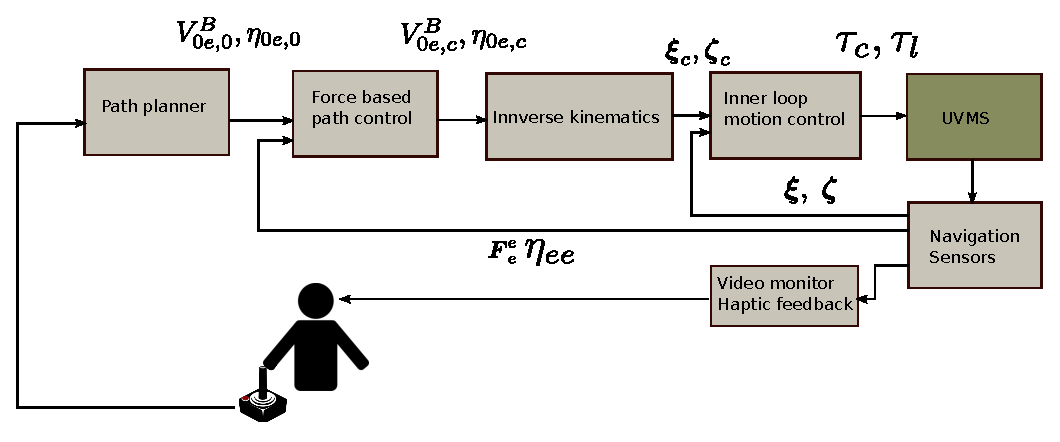
\includegraphics[scale=0.9]{./figures/control_structure.eps}
	\caption{Control structure}
	\label{fig:control_structure}
\end{figure}
In the third state of operation accurate position control is essential, and another approach is therefor proposed specifically for a hot stab operation in the test case below. 

\subsection{Motion Control}
The inner loop of the motion control is outside the scope of this text. For modelling and simulation purposes however, a control strategy based on feedback linearization is proposed, and implemented in SIMULINK in order to 
simulate the force control and the inverse kinematics. To simplify the implementation and analysis we use the model of the UVMS from \eqref{eq:dyn_with_current} split the input $\bs \tau$ into a cancelling term $\bs \tau_c$ and a 
linear control term $\bs \tau_l$ and use $\bs \tau_c$ to cancel out all the nonlinearities and terms including the current, similar to the control law proposed in \cite{foss_schjolberg_modelling}. The nonlinear canceling term yields

\begin{align}
\bs	\tau_{c} &=
  \bs C_{RB}(\zetab)\zetab + \bs g(\bs \eta) + \bs g_0 + \bs M_A \zetadotb_r  + \bs C_A(\zetab_r) \zetab_r + \bs D(\zetab_r) \zetab_r 
	\label{eq:nonlinear-cancelling}
\end{align}
While the linear control term is simply given as

\begin{align}
	\bs \tau_{l} & =\bs M(\bs q) \left(\bs K_{p} \tilde{\bs \zeta} + \dot{\bs \zeta}_{c} \right) \\
	\label{eq:linfeedback-lin}
	\tilde{\bs \zeta} &=\left(\bs \zeta_{c} - \bs{ \hat \zeta } \right)
\end{align}
Where $\bs{ \hat \zeta } $ is the measured or estimation of $\bs \zeta$, and $\bs K_{p}$ is a positive definite matrix. The resulting closed loop dynamics of the UVMS and low level control then yields
\begin{align}
	\bs M(\bs q)_{RB}\zetadotb =\bs M(\bs q) \left(\bs K_{p} \tilde{\bs \zeta} + \dot{\bs \zeta}_{c} \right) + (\bs J_{ge}^B)^T \bs F_{ee}
	\label{eq:linearized_feedback}
\end{align}
As long as there is no contact, the system is stable. This can be proved by looking at the error dynamics of the closed loop system \eqref{eq:linearized_feedback} for $\bs F_{ee}=0$.
\begin{align}
	\dot{\tilde{\bs \zeta}} & =- \bs K_{p} \tilde{\bs \zeta} 
	\label{eq:errordynamics}
\end{align}
Yielding asymtotic stability of the error.
It should be noted that the controller is only proposed for simulation purposes, in order to capture some of the dynamics of the system. Obtaining exact estimates of the nonlinear terms in \eqref{eq:nonlinear-cancelling} is, however, very difficult in real life, and it is thus difficult to guarantee stability.











\subsection{Kinematic Control}
An UVM system is kinematically redundant, meaning that it's configuration space is larger then the task space of the end effector. This is due to the 6 degrees of rotational and translational degrees of freedom of the underwater vehicle in addition to the degrees of freedom given by the number of manipulator joints. Because of this, each configuration of the end effector task space can be obtained by an infinite of configurations in the configuration space of the manipulator. 
As has been customary in robotics litterature, the mapping from the configuration space to the task space of the end effector\footnote{The task space is used to describe the configuration of the end effector relative to an inertial frame.} is done through the Jacobian, mapping the quasi-velocities of the system to the velocities of the end effector as described in \eqref{eq:body_jacobi}. The velocities can then be transformed to the time derivative of the general 
velocities, according to the analytical jacobian \eqref{eq:jacobian_a}, and then integrated to obtain the configuration $\bs \xi(t)$.

\begin{figure}[h!]
	\centering
	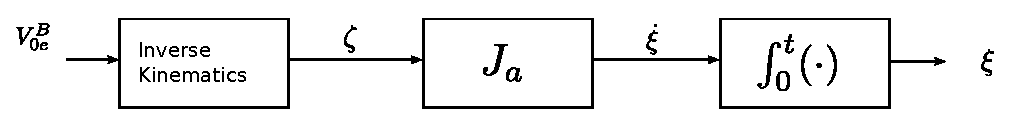
\includegraphics[scale=0.7]{./figures/inverse-kinematics1.eps}
	\caption{Transformation from end effector velocities to generalized coordinates of the UVMS}
	\label{fig:inverse1}
\end{figure}
The inverse kinematics is, in this context, described as the process of obtaining feasible quasi-velocities $\zeta$ from the desired end effector velocities. Due to the redundancy of the system, the set of feasible velocities $\zeta$ is not unique. In robotics litterature the Gradient Projection Method (GPM) is widely used in order to solve inverse kinematics. This method was first proposed in \cite{Liegeois1977}, and has later been developed and adapted my others.
Using the notation in this text, GPM by the following equation (\cite{Liegeois1977})

\begin{align}
	\bs	\zeta	&= \bs J^{+}\vb{0e}{B} + \left( \bs I -\bs J^{+} \bs J \right)k \nabla H
	\label{eq:gpm1}
\end{align}
Where the matrix $\bs J$ is the body geometric jacobian, as described in \eqref{eq:ee_velo_body}, and $\bs J^+ \in \Real{12\times 6}$ is the Moore-Penrose pseudo inverse of $\bs J$. $\left( \bs I - \bs J^{+}\bs J\right)$ projects the velocity matrix $k \nabla H$ into the null space of the jacobian. The vector $k \nabla H$ then describes the inner motion of the system, e.g. the motion that does not change the pose of the end effector (\cite{Liegeois1977} ).
Further, the vector $\nabla H$ is the gradient of a scalar cost function $H$ which is a measure of some performance criterion. For robot manipulator control, $H$ is typically used to avoid joint limits. The null projection of $\nabla H$
can be regarded as an inexact local solution to an optimization problem, where H is a convex function with $\bs \xi$ as the descicion variables. By choosing the gradient direction $\nabla H$ in the configuration space $\bs \xi$, as the null projected velocities gives an effective way of computing velocities to obtain the desired inner motion. The problem with GPM is that not all step lengths in the gradient direcion $\nabla H$ gives a feasible solutions (e.g. keeping the joint commands within the allowed joint limits). Therefore, the parameter k needs to be tuned to give a feasible solution. An efficient and robust method for scaling k is given in \cite{5723588} yielding

\begin{align}
	k&= - \frac{V_{m} - || \bs J^{+}\vb{0e}{B}|| }{||(\bs I - \bs J^{+}\bs J|| ||\left(\bs I - \bs J^{+}\bs J \right) \nabla H||} 
	\label{eq:k-scaling}
\end{align}
Where $V_{m}=||\bs \zeta_{max}||_{\infty}$, i.e. the absolute value of the largest allowed joint velocity of any joint. 




\subsection{Force Control}

Although no control method based on explicit force or impedance control is designed, it is useful to look at the forces of interaction between the end effector and the environment.
The forces on the end effector and the environment is analyzed in the task space, as observed by the end effector. Let the following define the forces in the end effector frame 
\begin{align}
	\bs F_{e}^e&=\begin{bmatrix} f_x & f_y & f_z & m_x & m_y & m_z \end{bmatrix}
	\label{eq:force_force}
\end{align}
$\bs F_{e}^e$ is therefor the same as $\bs F$ defined in \eqref{eq:jacobian_force} and can thus be mapped into the general forces $\taub$ by the transpose jacobian
\begin{align}
	\taub&=(\jb{ge}{B})^T\bs F_{e}^e
	\label{eq:jacobian-force2}
\end{align}

In robot manipulator control, it is customary to control the force between the end effector and the environment, either through direct force control or through controlling the apparent impedance between the end effector and the environment. This is typically done through hybrid impedance/force control, where the end effector is supposed to track a position or a force trajectory each in a subspace of the configuration space of a task frame \frame t. 
A typical application of this is a manipulator washing a car window, where the end effector is position controlled in the plane tangent to the window, while being impedance controled in the direction normal to the window. 
This kind of control scheme requires a priori knowledge of the geometry and environment impedance, and is thus challenging for a UVMS working in a generally unstructured environment. 
A control strategy which does not rely of this a priori knowledge is therefor proposed later in the paper.



























\subsection{Test Case: Semi Autonomous Hot Stab Operation}
A hot stab is a typical operation done by ROV's on subsea installations, which gives the opportunity to connect and disconnect different hydraulic components. 
The hot stab operation is in many ways analogous to the ``peg-in-hole'' problem which is widely studied in robotics litterature. The terms peg and hole will from now on refer to the hot stab tool, and the hole it is inserted into. 
Today, hot-stab is typically done by an operator controlling all of the degrees of freedom of the end effector, or directly in the joint space of the manipulator. This leads to difficulty in putting the peg in the hole, ecpecially 
with large delays in the human-UVMS-loop. 
The proposed strategy in this section is to lock most of the degrees of freedom to position set-points, and let the operator control a minimal set of DOFs. A fuzzy rule will handle the position set-points when the end effector is in 
contact with the environment. The concept is illustrated in Fig. \ref{fig:hot_stab2}.


\begin{figure}[h!]
	\centering
	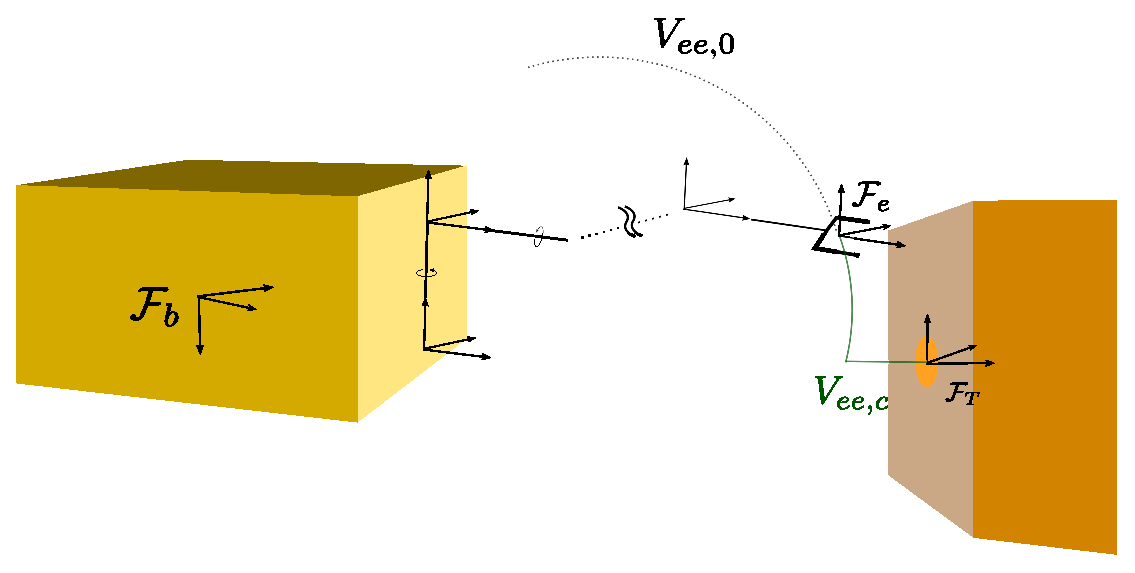
\includegraphics[scale=0.7]{./figures/uvms_hot_stab2.eps}
	\caption{Illustration of the UVMS in the transition between an operator ``flying'' the end effector according to $\bs V_{ee,0}$, and being position controlled in the $z,y,\theta $ and $ \psi$ direction in order to align with the task frame \frame t}
	\label{fig:hot_stab2}
\end{figure}
Further the sets $C$ and $NC$ are defined as

\begin{align*}
	C&=\{y_{ee},z_{ee},\theta_{ee},\psi_{ee}\} - \text{Compliant pose variables}
	\\
	NC&=\{x_{ee},\phi_{ee}\} \; \; \; - \; \text{ Non-Compliant pose variables}
\end{align*}
Where the pose variables above refer to the pose of \frame{ee} relative to the inertial frame. Further, the set-points $\bs \eta_{ee,0}$, given by the operator are good approximations to the pose of \frame{t} given in the inertial frame. Without loss of generality \frame{t} will be used as the inertial frame, and therefor the set-points are given as  
\begin{align}
C \subseteq	\bs \eta_{ee,0}=0
	\label{eq:subset}
\end{align}
A simple outer loop control law is proposed in order to assign a proper commanded velocity variables to the inverse kinematic control, and further, to the low level motion control

\begin{align}
	\bs V_{ee,c} &= \bs K_{1}\bs V_{ee,0} + \alpha \left( \bs F_{ee} \right) \bs K_{2} \tilde{\bs \eta}_{ee} 
	\label{eq:control_law1}
	\\
	\alpha &\in \left[ 0,1\right]
	\\
	\bs K_{1},\bs K_{2}&\in \Real{6 \times 6} \\
	\tilde{\bs \eta}_{ee,0}&= \bs \eta_{ee,0} - \widehat{\bs \eta}_{ee}
\end{align}
Where $\widehat{\bs \eta}_{ee}$ is the estimated or measured pose of the end effector. The matrices $\bs K_{1}$ and $ \bs K_{2}$ are positive semi-definite selection matrices, which selects the variables corresponding to $C$ and $NC$. $\bs K_{2}$ also weighs the contribution of the pose error.  

\begin{align}
	\bs K_{1} =\left[\begin{matrix}{}1 & 0 & 0 & 0 & 0 & 0\\0 & 0 & 0 & 0 & 0 & 0\\0 & 0 & 0 & 0 & 0 & 0\\0 & 0 & 0 & 1 & 0 & 0\\0 & 0 & 0 & 0 & 0 & 0\\0 & 0 & 0 & 0 & 0 & 0\end{matrix}\right]
	\label{eq:k1k2} \; , \; 
\bs K_{1} &=
\left[\begin{matrix}{}0 & 0 & 0 & 0 & 0 & 0\\0 & k_{22} & 0 & 0 & 0 & 0\\0 & 0 & k_{23} & 0 & 0 & 0\\0 & 0 & 0 & 0 & 0 & 0\\0 & 0 & 0 & 0 & k_{25} & 0\\0 & 0 & 0 & 0 & 0 & k_{26}\end{matrix}\right]
\end{align}
The scalar function $\alpha$ are weighting the last term in \eqref{eq:control_law1} based on a fuzzy rule described later. Taking $\alpha = 1$, the control law in \eqref{eq:control_law1} acts as a PI controller on the end effector velocity $\bs V_{ee}$. Where the pose is regarded as the integral of the velocity. Although this is not true in general, since the angular velocities $p_{ee}, q_{ee}$ and $r_{ee}$ in  $\bs V_{ee}$ are quasi-velocities, it can be shown that it is a good approximation close to the end effector pose $\phi_{ee} = \theta_{ee}=\psi_{ee}=0$. The approximation of transformation matrix $\bs T$ from body velocities to euler angle rates, for small angles $\delta \phi, \delta \theta$ and $\delta \psi$ is given in \cite{fs} as

\begin{align}
	\bs T(\delta \bs \eta_{2}) &\approx \begin{bmatrix} 1 & 0 & \delta \theta \\ 0 & 1 & -\delta \phi \\ 0 & \delta \phi & 1 \end{bmatrix}	
	\label{eq:linearized-transformation}
	\\
	\bs T(\delta \bs \eta_{2}) \big|_{\eta_{2}=0} &\approx \bs I_{3 \times 3}
	\label{eq:linearized-transformation2}
	\\
	\dot{\bs \eta}_{ee}&\approx\bs T(\delta \bs \eta_{2}) \begin{bmatrix} p \\ q \\ r\end{bmatrix}
	\\
	\Rightarrow \dot{\bs \eta}_{ee}&\approx \begin{bmatrix} p \\ q\\  r\end{bmatrix}
\end{align}
It is important to notice that the euler representation gives singularities for certain configurations. Therefor, in a robust implementation, quaternions could be used instead. For the purpose of analysis, however, the euler angles have a more intuitive interpretation, and will be used throughout this section.
Besides acting as a PI controller, the last term in \eqref{eq:control_law1} can also be seen as a path correction term, correcting the velocity $\bs V_{ee,0}$ when deviating from the desired path. When the end effector is in the free flying state, this path correction is done by the operator, correcting the velocity based on observed deviations through e.g. video feedback. 

It is reasonable to assume that the hot-stab system is designed so that it allows a slight error of the positions in $C$, for instance through making the insertion point bigger than the size of the peg, and gradually decreasing in size to make the peg fit. If the $C$ -positions are commanded correctly relative to \frame t the simple PI design of \ref{eq:control_law1} with $\alpha=1$ is sufficient. However, small deviations can occure, either a result of the low level control loop's inability to track the commanded velocity, or by a slight misalignment of the task frame \frame t relative to the physical task. As a result of this, the set points in $C \subseteq \bs \eta_{ee,0}$ can cause the end effector to be commanded (through $\bs V_{ee,c}$) to a set point causing collision with the rigid structure of the environment. This can be seen from \eqref{eq:control_law1}, where a nonzero $\bs K_{2}\tilde{\bs \eta}_{ee}$ commands the end effector to keep a velocity in a direction blocked by the rigid environment.

More generally, the directions controlled purely by velocity will be more compliant to interaction with the environment, as long as the desired velocity is zero. Although an interaction with the environment causes the end effector to be slightly off the planed velocity trajectory, it will only regulate the velocity to 0, and not try to push on the environment due to a position offset. If the position correction term is used, (corresponding to a nonzero $\alpha$)
the end effector will be commanded to push on the environment, if the set-points are slightly off the free motion path. A fuzzy tuning rule for $\alpha$ is therefor proposed to stop the position correction term in \eqref{eq:control_law1} when a the magnitude of the force $\bs F_{ee}$ has reached a certain threshold. 



Let the the p-norm of $\bs F_{ee}$ for $p=2$ be denoted $$F_n=||\bs F_{ee}||_{2}$$ The scalar function $F_{n}$ is then a measure of the total amount of force acting on the end effector. The proposed tuning of $\alpha$ is listed in algorithm \ref{alg:alt1} 
	\begin{Algorithm}{12cm}
	\caption{Fuzzy tuning rule for $\alpha$ \label{alg:alt1}}
\begin{algorithmic}
	\REQUIRE $alpha$ initialized to 1
	\IF{$\alpha$ is already 0}
    \STATE    $\alpha=0$
		\ELSIF{$F_{n} < f_{1}$}
        \STATE $\alpha=1$
    \ELSE
        \STATE $\alpha = 0$
    \ENDIF
\end{algorithmic}
\end{Algorithm}

where $f_{1}$ is the threshold force, which is a tuning parameter of the problem. It should be noted that if $\alpha$ has already been set to 0, it wont be reset to 1 automatically. This is to avoid jittering between the states where the forces are above and below the threshold. It is also assumed that the mechanics of the hot stab, allows the peg to be guided into the hole, as long as it is entering it without too much deviation.  By tuning $\alpha$ according to algorithm \ref{alg:alt1}, the end effector is controlled to the desired position $\bs \eta_{ee}$ as long as the force on the end effector is below a certain threshold. If the peg is entering the hole, without being too misaligned, it should be able for an operator to control the insertion of the peg along the $x_{ee}$ axis, without causing too much force on the end effector. 























